\documentclass[main]{subfiles}
\begin{document}
\chapter{问题及算法叙述}\label{chp:prob_setup}
\section{问题}
\paragraph{记号: }
我们记无噪音的数据矩阵为 $Y \in \mathbb{R}^{d\times n}$,  $Y$ 的每一列都属于$L$
个子空间的交
$$\mathcal{S}_1 \cup \mathcal{S}_2 \cup...\cup \mathcal{S}_L.$$
并且都是单位向量
\footnote{单位化的条件能使后面的证明叙述简洁,不过我们的结论能拓展到一般的情形只需要对后面给出的条件稍作修改。}。

每个子空间 $\mathcal{S}_{\ell}$ 的维度是 $d_{\ell} \le d$ 并且有 $n_{\ell}$
个采样点,满足$n_1 +n_2+...+n_L=n$. 我们观察到的带噪音的数据矩阵为 $X = Y+Z$,
其中 $Z$ 是噪音矩阵. 令 $Y^{(\ell)}\in \mathbb{R}^{d\times n_{\ell}}$ 表示 
$Y$ 中属于 $\mathcal{S}_{\ell}$ 的列组成的矩阵,相应的我们可以定义 $X^{(\ell)}$ 和 $Z^{(\ell)}$.
不失一般性地,令$X=[X^{(1)},X^{(2)},...,X^{(L)}]$ ,即采样点按照子空间聚在一起.
花体字母 $\mathcal{X},\mathcal{Y_{\ell}}$ 表示对应矩阵(即 $X$ 和 $Y^{(\ell)}$)的所有列向量组成的集合。

对任一矩阵 $X$, $\mathcal{P}(X)$ 表示其所有列向量张成的对称凸包,即
$\mathcal{P}(X) = \mathrm{conv}(\pm \mathcal{X})$。简记
$\mathcal{P}_{I^c}^{(\ell)} := \mathcal{P}(X_{I^c}^{(\ell)}), \mathcal{Q}_{I^c}^{(\ell)} :=
\mathcal{P}(Y_{I^c}^{(\ell)})$。$\mathbb{P}_{\mathcal{S}}$ 和
$\mathrm{Proj}_{\mathcal{S}}$ 表示子空间 $\mathcal{S}$
的投影矩阵和投影算子。我们使用$X_i$ 表示矩阵$X$ 的第$i$列,$X_i^T$ 表示矩阵转置后的第$i$列, $X_I$
表示将$X$矩阵的列按照指标集$I$取出后组成的子矩阵.
同理$X^T_I$是转置后的子矩阵。定义$\|X\|_{2, 1}:= \sum_i \|X_i\|_2$ ,
$\norm(X)$是将$X$的每一列归一化($X_i \neq \mathbf{0}$),$\langle X, Y \rangle
:= \tr(X^T Y)$。

\section{初步聚类}
我们第一步是将数据点分成若干组,使得每一组里的点属于同一个子空间。为了做到这点
必须利用数据的空间性质。事实上,当采样点充分且子空间之间分离性较好时,一个数据点的邻居很可能
与它是同一类。这种性质在很多实际应用中天然满足,比如运用分割中,位置比较接近的点很可能来自
同一个物体。

然而如果只考虑数据点的邻居,这无疑忽略了线性空间的性质,于是我们定义一个新的点到点集距离:
\begin{definition}[点到空间距离]\label{def:space_distance}
  设$x\in \R^d, X\in \R^{d\times n}$,$k$为给定正整数,我们有距离函数
  $$ d(x, X, k) = \begin{cases} \|x -\cP_{U_{1:k}} x\|_2 & \text{非仿射空间}\\
    \|x - \cP{\tU_{1:k}} x\|_2 & \text{仿射空间} \end{cases},$$
  其中$U$为$X$svd的左奇异向量矩阵,$\tU$为$\tX=X-\frac{1}{n}\sum_{i=1}^n
  X_i$的svd左奇异向量矩阵。
\end{definition}
如果我们已经有了$n$个点那么就可以再取下一个离点集最近的点。

下一个问题是每一组应该选取多少个点,如果取得过少,不能很好的发挥Group LASSO
和Multitasking 的作用,如果过多,很可能有错误点。

\begin{algorithm} \caption{拓展最近邻}
  \begin{algorithmic} \label{alg:nsn}
    \Require $n$ 个样本点 $\mathcal{X} = \{x_1,\ldots,x_n\}$, 所需邻居的个数
    $K$, 邻域子间维度 $k_{\max}$.
    \Ensure 所有样本点的分组$\Omega$
    \State $m=1$
    \Repeat
      \State 从$\cX$中任选一个点$x_0$
      \State $\set{S}_m \gets \{x_0\}$ \Comment{$x_0$点张成的子空间}
      \For {$k = 1,\ldots,K$} \Comment{依次将最近邻加入子空间集合}
        \State $x^* \gets \argmin_{x \in \cX  \setminus \set{S}_m} d(x, S_m,
        k_{\max})$
        \State $\set{S}_m \gets \set{S}_m \cup \{x^*\}$
      \EndFor
      \State $\Omega \gets \Omega \cup \set{S}_m$
      \State $cX \gets \cX \setminus \set{S}_m$
      \State $m=m+1$
    \Until{$\cX$ 为空}
  \end{algorithmic}
\end{algorithm}

算法 \ref{alg:nsn} 将样本点分成SN collects $K$ neighbors sequentially for each point. At each step $k$, a
$k$-dimensional subspace $\set{U}$ spanned by the point and its $k-1$ neighbors
is constructed, and the point closest to the subspace is newly collected. After
$k \ge k_{\max}$, the subspace $\set{U}$ constructed at the $k_{\max}$th step
is used for collecting neighbors. At last, if there are more points lying on
$\set{U}$, they are also counted as neighbors. The subspace $\set{U}$ can be
stored in the form of a matrix $U \in \mathbb{R}^{p \times
  \text{dim}(\set{U})}$ whose columns form an orthonormal basis of $\set{U}$.
  Then $\|\proj_{\set{U}} y_j\|_2$ can be computed easily because it is equal
  to $\|U^\top y_j\|_2$. While a naive implementation requires $O(K^2pN^2)$
  computational cost, this can be reduced to $O(KpN^2)$, and the faster
  which solve a convex program with $N^2$ variables and $pN$ constraints.

\section{Group LASSO 和 Multitasking}
原有的 SSC 方法,主要求解下面的优化问题
\begin{equation}\label{eq:SSC}
  \begin{aligned}
    \min_{c_i} \; \|c_i\|_1 \quad s.t. \quad &x_i=X_{I^c}c_i,
  \end{aligned}
\end{equation}
for each data point $x_i$. Solutions are arranged into matrix $C=[c_1,...,c_N]$, then spectral clustering techniques such as \cite{ng2002spectral} are applied on the affinity matrix $W=|C|+|C|^T$ ($|\cdot|$ represents entrywise absolute value). Note that when $Z\neq 0$, this method breaks down: indeed \eqref{eq:SSC} may even be infeasible.

To handle noisy $X$, a natural extension is to relax the equality constraint in \eqref{eq:SSC} and solve the following unconstrained minimization problem instead \cite{elhamifar2012ssc_journal}:
\begin{equation}\label{eq:Lasso}
\begin{aligned}
\min_{c_i} \; &\|c_i\|_1+\frac{\lambda}{2}\|x_i-X_{I^c}c_i\|^2.
\end{aligned}
\end{equation}
We will focus on Formulation~\eqref{eq:Lasso} in this paper. Notice that \eqref{eq:Lasso} coincides with standard LASSO. Yet, since our task is subspace clustering, the analysis of LASSO (mainly for the task of support recovery) does not extend to SSC. In particular, existing literature for LASSO to succeed requires the dictionary $X_{I^c}$ to satisfy the Restricted Isometry Property~\cite[RIP for short;][]{candes2008RIP} or the Null-space property~\cite{donoho2006BPDN},  but neither of them is satisfied in the subspace clustering setup.\footnote{As a simple illustrative example, suppose there exists two identical columns in $X_{I^c}$, which violates RIP for 2-sparse signal and has maximum incoherence $\mu(X_{I^c})=1$.}

In the subspace clustering task, there is no single ``ground-truth'' $C$ to compare the solution against. Instead, the algorithm succeeds if each sample is expressed as a linear combination of samples belonging to the same subspace, as the following definition states.
\begin{definition}[LASSO Subspace Detection Property]\label{def:lasso_detection}
We say the subspaces $\{\mathcal{S}_{\ell}\}_{\ell=1}^{k}$ and noisy sample points $X$ from these subspaces obey LASSO subspace detection property with parameter $\lambda$, if and only if it holds that for all $i$, the optimal solution $c_i$ to \eqref{eq:Lasso} with parameter $\lambda$ satisfies:\\
\indent (1) $c_i$ is not a zero vector, i.e., the solution is non-trivial,
\indent (2) Nonzero entries of $c_i$ correspond to only columns of $X$ sampled from the same subspace as $x_i$.
\end{definition}
This property ensures that the output matrix $C$ and (naturally) the affinity matrix $W$ are exactly block diagonal with each subspace cluster represented by a disjoint block.  The property is illustrated in Figure~\ref{fig:SEP}. For convenience, we will refer to the second requirement alone as ``\emph{Self-Expressiveness Property}''~(SEP), as defined in \cite{elhamifar2012ssc_journal}.

Note that the LASSO Subspace Detection Property is a strong condition. In practice, spectral clustering does not require the exact block diagonal structure for perfect segmentation in our simulation section for details). A caveat is that it is also not sufficient for perfect segmentation, since it does not guarantee each diagonal block forms a connected component. This is a known problem for SSC \cite{nasihatkon2011graph}, although we observe that in practice graph connectivity is usually not a big issue. Proving the high-confidence connectivity (even under probabilistic models) remains an open problem, except for the almost trivial cases when the subspaces are independent \cite{liu2013LRR, wang2013provable}.

\begin{figure}
  \centering
  % Requires \usepackage{graphicx}
  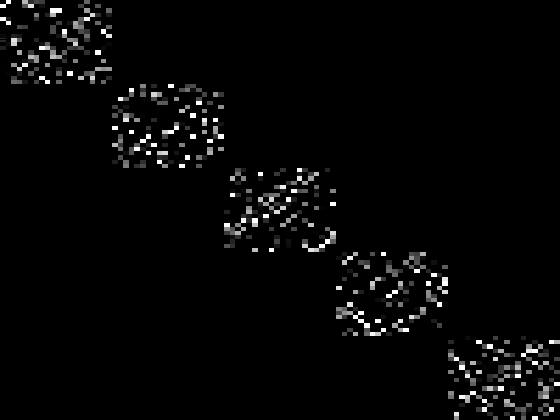
\includegraphics[width=0.35\linewidth]{pics/SEP.png}
  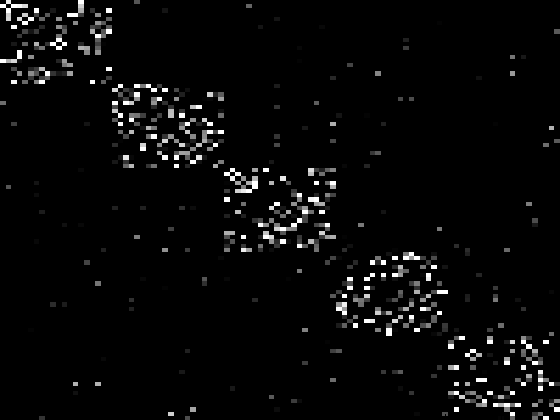
\includegraphics[width=0.35\linewidth]{pics/ViolateSEP.png}\\
  \caption{Illustration of LASSO-Subspace Detection Property/Self-Expressiveness Property. \textbf{Left:} SEP holds. \textbf{Right:} SEP is violated even though spectral clustering is likely to cluster this affinity graph perfectly into 5 blocks.}\label{fig:SEP}
\end{figure}

\paragraph{Models of analysis: }
Our objective here is to provide sufficient conditions upon which the LASSO subspace detection properties hold in the following four models. Precise definition of the noise models will be given in Section~\ref{sec:main}.

\begin{tabular}{ll}
  $\bullet$ fully deterministic model;\\
  $\bullet$ deterministic data with random noise;\\
  $\bullet$ semi-random data with random noise;\\
  $\bullet$ fully random model.
\end{tabular}
\end{document}
